\section{Summary of ADS-B Cleaning Methods, work flow}

\subsection {Data Quality Issues in ADS-B Surveillance}

Real-world ADS-B data often contain a considerable amount of noise and anomalous errors. Several studies have conducted in-depth analyses of these issues. For instance, Tabassum et al. \cite{8102001} systematically demonstrates various types of anomalies found in ADS-B messages, while \cite{8569833} and \cite{Olive_Krummen_Figuet_Alligier_2025} provide detailed examinations of noise sources and error mechanisms within crowdsourced datasets. These studies collectively indicate that ADS-B data quality is heavily influenced by factors such as hardware performance, signal environment, and network structure, resulting in inconsistencies and unreliability across raw observations.

In general, the quality issues of ADS-B data can be categorized into four dimensions:

(1) \textbf{Completeness}: ADS-B data often suffer from message loss, missing fields, and update interruptions, leading to temporal or spatial discontinuities in flight trajectories. Such problems are mainly caused by variations in receiver performance, signal attenuation, and the instability of crowdsourced networks, resulting in insufficient data coverage.

(2) \textbf{Consistency}: Some data exhibit internal contradictions in temporal, spatial, or physical attributes, such as out-of-order timestamps, abrupt altitude jumps, or unrealistic speed values. These issues typically arise from clock drift, decoding errors, or improper data aggregation from multiple sources, undermining the logical coherence of trajectories.

(3) \textbf{Accuracy}: Systematic deviations may exist between the reported ADS-B values and the actual flight states—for example, discrepancies between barometric and geometric altitude or significant errors in reported positions and speeds. The main causes include quantization errors, receiver precision limitations, and environmental interference.

(4) \textbf{Reliability}: ADS-B datasets may contain random noise, falsified messages, or artifacts introduced by multi-source fusion, all of which degrade the credibility and usability of the information. Such reliability issues are particularly prominent in open, crowdsourced data collection environments, increasing uncertainty in subsequent analyses and modeling.

In summary, various types of errors may occur throughout the collection, transmission, and aggregation of ADS-B data. Without proper treatment, these problems can severely affect the performance of downstream algorithms and compromise the reliability of analytical results. Therefore, systematic data cleaning and quality control are essential prerequisites to ensure the usability and accuracy of ADS-B data for further research and algorithmic applications.

\subsection {Data cleaning methods}
\subsubsection{Task-Oriented Filtering}
Filtering ADS-B data is typically the initial step in data cleaning. Depending on the research objectives and application scenarios, most studies perform preliminary filtering of raw ADS-B data before analysis to ensure that the data used are relevant and representative. Common filtering strategies can be broadly categorized into range-based filtering and attribute-based filtering.

\textbf{(1) Range-Based Filtering}

This approach primarily selects ADS-B data based on temporal or spatial ranges. Temporal filtering can limit the data to specific seasons, dates, or time periods to match the study timeframe. Spatial filtering focuses on particular routes, airspaces, or airport operations. Additionally, trajectories within specific geographic boundaries (e.g., latitude/longitude ranges or airspace altitude layers) may be extracted to construct local operational networks or airspace models.

\textbf{(2) Attribute-Based Filtering}

Beyond temporal and spatial constraints, researchers may remove trajectories that are irrelevant or do not meet task-specific criteria. This type of filtering is often based on flight rules, operational states, aircraft types, or flight phases. For example, Dhief et al. \cite{dhief2021tree} excluded flights operating under Visual Flight Rules (VFR) in a go-around behavior study. Similarly, Liu et al. \cite{LIU2024104652id} filtered trajectories under consistent weather conditions in their study on taxiing optimization at Shenzhen Bao’an Airport to reduce the influence of weather variations and runway configurations.

\subsubsection{Outlier Detection and Removal} 

After the initial filtering, it is usually necessary to identify and remove outliers in order to ensure the reliability of subsequent analyses. \cite{olive2024filtering} review summarized and investigated common methods for outlier detection and handling. Common outlier handling methods include the removal of entire trajectories, local cleaning of individual abnormal points, and automated detection based on clustering or deep learning techniques.

The most common approach is the removal of entire trajectories. Outlier trajectories can arise from various reasons, the most frequent being incomplete data, such as trajectories with too few sampling points to accurately represent the flight process, which need to be excluded.

For trajectories that are generally valid but contain a few abnormal points, researchers typically perform local cleaning. Common types of noise include duplicate points and physically impossible “jump points.” Methods such as Gaussian filtering or particle filtering are often used to smooth trajectories and correct these anomalies.

In addition, density-based clustering algorithms like DBSCAN are widely applied in outlier detection and cleaning. DBSCAN can automatically identify outliers based on point density and separate them from normal trajectories, allowing simultaneous trajectory clustering and outlier removal. Compared to traditional filtering methods, DBSCAN offers greater flexibility and automation, particularly for trajectory data with uneven spatial distribution.

Autoencoders (AE), as a deep learning approach, can also be employed for anomaly detection. AE learns typical patterns of normal trajectories during training, and abnormal trajectories or points usually exhibit larger reconstruction errors. These errors can then be used to identify and remove outliers. AE is capable of capturing nonlinear relationships in data, making it particularly suitable for high-dimensional and time-series ADS-B trajectory data, and it can be combined with filtering or clustering methods for more precise cleaning.


\subsubsection{Interpolation and resampling} 

In ADS-B data processing and trajectory reconstruction, interpolation and resampling are two essential preprocessing techniques.
Interpolation focuses on repairing missing data points and ensuring trajectory continuity, while resampling aims to unify the temporal or spatial distribution of data, thereby improving the stability of subsequent analysis and model training.
Since both techniques are often applied together in practice, they are presented here in an integrated discussion.

\textbf{(1)Interpolation}

The objective of interpolation is to estimate missing values between known points, thereby converting discrete trajectories into continuous and smooth curves.
Depending on the fitting principle, common interpolation methods can be categorized into three groups:

\textbf{Linear and Polynomial Interpolation}
This is the most widely used class of interpolation techniques, which assumes that variations between adjacent points follow a linear or low-order polynomial relationship.
These methods are computationally efficient and suitable for short time intervals or smooth motion, but their ability to capture nonlinear behavior—such as turning or climbing—is limited.
Representative methods include linear interpolation \cite{lindner2021aircraft} and polynomial interpolation.

\textbf{Spline-Based Interpolation}
Spline methods fit piecewise polynomial functions while maintaining continuity at segment boundaries, achieving higher smoothness and stability.
Typical examples include linear spline interpolation \cite{sun2019wrap}, cubic spline interpolation \cite{shafienya20224d}, and piecewise cubic Hermite interpolation (PCHIP) \cite{10311324}, which introduces shape-preserving constraints to prevent unrealistic oscillations.
Compared with simple linear methods, spline-based interpolation offers superior smoothness and shape retention, making it widely used for flight trajectory reconstruction and long-duration signal completion.

\textbf{Spatially Adaptive Interpolation}
This approach ensures consistent spatial resolution along the trajectory, achieving globally uniform point density while preserving geometric accuracy and spatial consistency.

\textbf{(2) Resampling Methods}

Resampling aims to transform irregularly spaced ADS-B data into a unified format suitable for downstream analysis and model input.
According to the dimension of unification, resampling techniques can be classified into four categories:

\textbf{Fixed-Time Interval Resampling}
This method extracts or generates data points at a fixed temporal interval, ensuring uniform time distribution along the trajectory.
It is the most fundamental form of temporal standardization, with sampling intervals ranging from one second \cite{WANG2020101840} to several minutes \cite{vos2024transformer}, depending on the temporal resolution required by the study.

\textbf{Trajectory Feature-Based Resampling}
Instead of relying on fixed intervals, this approach resamples according to geometric characteristics such as turning points or curvature changes, thereby reducing redundancy while preserving essential trajectory features.The representative algorithms are: RDP Algorithm (Douglas–Peucker) \cite{SCHULTZ2022102164}: Iteratively removes points with distances below a given threshold from the line connecting the start and end points, retaining only key inflection points. This reduces data volume while maintaining the overall geometric structure of the trajectory. 
Fixed Number of Inputs algorithm: Uses interpolation to map each trajectory into a fixed number of points, ensuring consistent input dimensions for deep learning models such as autoencoders \cite{olive2018detecting} and Transformers \cite{BAO2024102667}.

\textbf{Spatial or Curve-Based Resampling}
This category focuses on spatial uniformity or curve smoothness.
Points are extracted along the trajectory at fixed spatial intervals to achieve uniform spatial density, which is particularly useful for spatial analysis tasks such as airport vicinity trajectory density mapping or taxiway path planning, where uneven temporal sampling may otherwise cause spatial distortion.

\subsubsection{Smoothing}

After temporal or spatial resampling, researchers often apply trajectory smoothing to further suppress noise, reduce trajectory jitter, and preserve the essential motion trend, thereby providing more reliable inputs for subsequent analysis and model construction.
According to their underlying principles and computational characteristics, trajectory smoothing methods can generally be categorized into three groups:

\textbf{(1) Model-based filtering methods}

These methods rely on state-space or probabilistic estimation models to describe the relationship between the aircraft’s true motion states and observational noise, achieving optimal trajectory estimation and smoothing.
Representative algorithms include the Kalman Filter \cite{LU2021102970} and Extended Kalman Filter, which obtain optimal state estimates by minimizing the covariance of recursive estimation errors. Owing to their strong dynamic modeling capability and physical interpretability, such methods are widely used for aircraft state estimation and altitude smoothing tasks.

\textbf{(2) Signal processing–based filtering methods}

In this approach, the trajectory is treated as a time-series signal, and digital filters are employed to suppress undesired frequency components, thus achieving trajectory smoothing.
Typical examples include the finite impulse response (FIR) low-pass filter \cite{churchill2019clustering}, the Exponential Moving Average (EMA) algorithm \cite{ZHU2023102473} , and the bilateral window averaging method \cite{7549107}. By convolutional or recursive operations, these methods effectively remove oscillatory noise from uniformly sampled trajectories.

\textbf{(3) Curve-fitting and geometric-statistical methods}

These methods approximate the entire trajectory using mathematical curves or geometric-statistical representations to achieve global-level smoothing, producing continuous and geometrically consistent trajectories.
For instance, the smoothing cubic spline \cite{alligier2018learning} is a variational fitting technique that balances data fidelity and smoothness through an optimized regularization parameter. The Hough voting algorithm \cite{LIU2024104652}, based on the global geometric consistency of trajectories, maps local trajectory features into a parameter space and serves as a common tool for geometric trajectory reconstruction.

\subsubsection{ADS-B data cleaning pipeline}

Overall, ADS-B data cleaning typically follows a logical progression from macroscopic filtering to microscopic refinement.
% TODO: \usepackage{graphicx} required
\begin{figure}
	\centering
	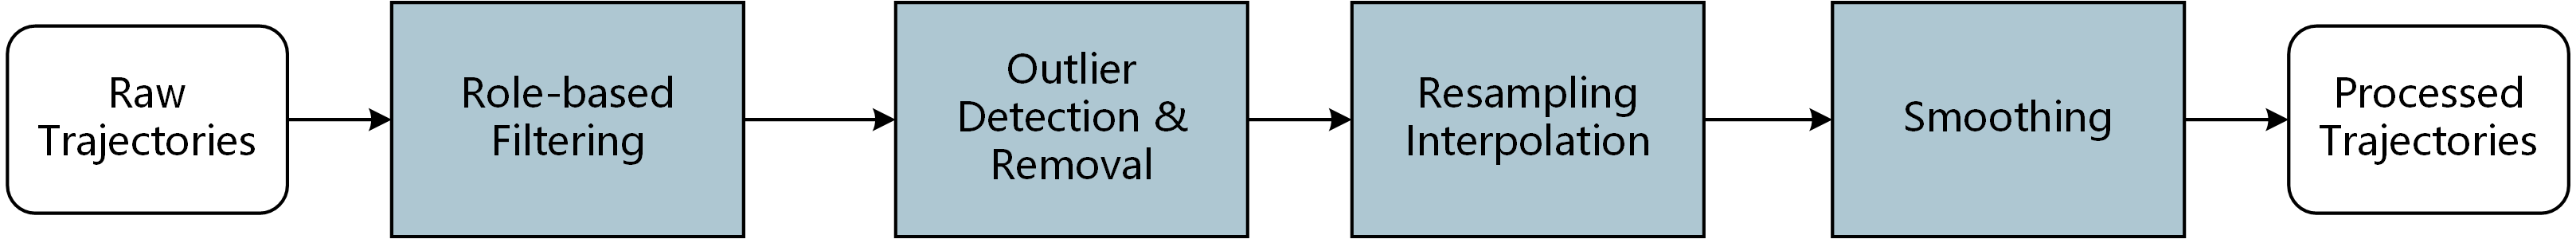
\includegraphics[width=0.8\linewidth]{pipeline}
	\caption[Figure 3]{Pipeline of ADS-B data cleaning}
	\label{fig:Pipeline}
\end{figure}

As illustrated in Figure \ref{fig:Pipeline}, the cleaning process generally consists of the following steps:

First, the raw ADS-B data are filtered by temporal, spatial, and flight-related attributes according to the research objectives, in order to extract a subset that meets the analysis requirements.
Next, preliminary denoising is performed, including duplicate removal, elimination of trajectories with excessive missing data, and correction of abrupt anomalies, thereby improving data completeness and consistency.
On this basis, interpolation and resampling are applied to fill missing values and to unify the temporal or spatial resolution, providing a structured foundation for subsequent algorithmic processing.
Finally, trajectory smoothing is carried out to further suppress residual noise and random jitter, extracting the core motion trends that reflect the true flight dynamics.

In recent years, several open-source tools have provided comprehensive support for implementing the above data-cleaning procedures. Among them, the Traffic Library \cite{olive2019traffic} has been widely adopted. It offers ready-to-use implementations for each stage of the workflow, greatly simplifying the preprocessing of ADS-B data. Researchers can transform raw data into high-quality trajectories without developing low-level algorithms manually, which significantly lowers the technical barrier to aviation data processing and allows greater focus on downstream analytical tasks.

It should be noted that the above workflow is derived from a systematic review and comparative analysis of the collected papers. However, the survey reveals significant inconsistencies in how data-cleaning procedures are described across studies. Some works mention only general terms such as “filtering” or “pre-processing” without detailing the specific methods or parameter configurations. This lack of transparency and consistency undermines the reproducibility and comparability of research outcomes and may also affect the reliability of conclusions regarding algorithmic performance.

\subsection{Analysis of Data Cleaning Operations}

The previously discussed data cleaning procedures can enhance the completeness, consistency, accuracy, and reliability of ADS-B data. However, their impact on downstream algorithms is complex and multifaceted.

Outlier Removal: Eliminating outliers helps filter noise and improve data purity, yet misjudgments may remove legitimate maneuvers (e.g., temporary avoidance), thereby reducing the accuracy of flight pattern modeling. Excessive removal of marginal data can also reduce the sample size and weaken the representativeness of rare conditions such as adverse weather or remote airspace. Moreover, among the two methods introduced earlier, DBSCAN is sensitive to uneven trajectory densities and may misclassify sparse but normal points as anomalies. The Autoencoder (AE), on the other hand, relies on sufficient and high-quality normal data for training; any bias in the training set may shift the anomaly detection threshold, causing normal trajectories to be incorrectly flagged as outliers and introducing additional judgment errors.

Interpolation and Resampling: These techniques are commonly used to fill missing points and unify temporal resolution, thereby improving the continuity and comparability of trajectories. However, excessive or improper interpolation may smooth out genuine micro-maneuvers (e.g., speed adjustments), while resampling, as a data transformation process, may introduce artificial variations in speed and acceleration. Such alterations can distort the instantaneous motion parameters of aircraft, making it difficult for models that depend on short-term motion states (e.g., LSTM-based trajectory prediction) to capture key dynamics, thus increasing prediction errors. In addition, interpolation may blur instantaneous proximity between aircraft, reducing the sensitivity of conflict detection and risk identification.

Smoothing: Kalman or low-pass filters effectively suppress high-frequency jitter in positional data, producing smoother trajectories and facilitating the calculation of derived features such as heading and curvature. Nevertheless, smoothing can weaken sharp trajectory characteristics, such as the precise onset and recovery points of turns, which may negatively affect maneuver-based anomaly detection (e.g., go-around identification) and flight phase classification models.

Overall, ADS-B data cleaning is a crucial step in improving data integrity and reliability. However, as the above limitations indicate, over-cleaning may remove essential flight characteristics, while insufficient cleaning may fail to meet the quality requirements for algorithmic processing. Both extremes can adversely affect downstream analysis and model performance.

Therefore, in practical applications, researchers need to balance data fidelity and usability when designing preprocessing pipelines. In the following chapters, the influence of different cleaning strategies on algorithm performance will be quantitatively evaluated through experiments.
